\chapter{Qweak Main Cerenkov Detector}\label{CHP_V}

This chapter explains the implementation of the QWeak main detector in
the simulation, including the physical layout and material properties
as well as event data readout.  The chapter also provides a discussion
(code trace) of the way GEANT4 handles the optical transport
physics. This is discussed somewhat in the GEANT4 physics reference
manual~\cite{tn:GEANT4PRM}\footnote{{\tt
http://geant4.web.cern.ch/geant4/UserDocumentation/UsersGuides/\\PhysicsReferenceManual/html/index.html}},
but not in very much detail. Here, we verify the physics by looking at
code itself and relating it to the material and geometry
specifications made in the QWeak simulation. For the QWeak main
detectors, the two most relevant GEANT4 classes which specify the
physics are {\it G4Cerenkov} and {\it G4OpBoundaryProcess}.

The overal detector geometry and properties are implemented in the
class {\it QweakSimCerenkovDetector}. However, some of the detector
material properties, the data readout and the sensitivity are
implemented in combination with other classes listed in
table~\ref{tbl:V-I}, some of which serve multiple objects at the same
time.  The relation to and use of each of these classes for the main
detectors is discussed in separate sections.

\section{Detector Implementation}

The detector atributes or properties that are currently implemented
are listed in table ~\ref{tbl:V-II}. Each property has one or several
sections devoted to it, describing the details of the code.  Please
refer to the code listings provided at the end of each chapter for
each class. Components placed inside another volume (their respective
parent volume) are positioned with respect to the center of the parent
volume.

Aside from the constructor and destructor, there are 16 public access
member functions declared in the header.  Shown in
fig.~\ref{fig:V-SC-1} (lines 26 trough 46), they provide mechanisms to
control the detector position, construct or remove the detector
geometry (called by {\it QweakSimDetectorConstruction},
p.~\pageref{QweakSimDetectorConstruction}), update the geometry
between runs, as specified by the position variables passed to the
setters (lines 34 through 38), and provide access to the sensitive
logical and physics volume which are private data members used by
the Geant4 run manager. The function {\it CerenkovGeometryPVUpdate} 
provides a way to change the geometry between runs, using the input
({\em *.mac}) files (see p.~\pageref{batchIII}). The meat of the detector
implementation is handled in the function {\it ConstructComponent}.
Some of the functions, such as {\it DefineCerenkovGeometry} are currently
not used. 

\begin{table}
\begin{center}
\begin{tabular}{lll}
\hline 
 {\bf Object / Property} &  {\bf Class}                     & {\bf Use}\\
\hline 
 Quartz Sensitive Volume &  Cerenkov\_DetectorSD          & event definition and \\
                         &                                & sensitivity cuts \\
                         &                                & \\
 PMT Sensitive Volume    &  CerenkovDetector\_PMTSD       & event definition and \\
                         &                                & sensitivity cuts \\
                         &                                & \\
 Material Type           &  Material                      & obtain material \\
                         &                                & properties\\
                         &                                & \\
 Event Info Container    &  UserInformation               & pass event information \\
                         &                                & between objects\\
                         &                                & \\
 Partcile Step Info      &  SteppingAction                & extract information for\\ 
                         &                                & each particle step\\ 
                         &                                & \\
 Partcile Track Info     &  trackingAction                & extract information for\\ 
                         &                                & each particle track\\
                         &                                & (used for secondaries)\\ 
                         &                                & \\
 Event Readout           &  UserCerenkov\_MainEvent	  & define the tree structure \\
                         &  UserCerenkov\_OctantEvent	  & for the Cerenkov and PMT\\
                         &  UserCerenkov\_DetectorEvent   & data readout\\
                         &  UserCerenkov\_PMTEvent        & \\
 \hline
\end{tabular}
\end{center}
\caption{List of detector and connected classes which 
         are currently implemented.}
\label{tbl:V-I}
\end{table}

\subsection{Geometry}

The detector geometry is specified via the use of containers within
containers. The configuration is shown in figure~\ref{fig:VOLCONT}.

\subsubsection{Master Container}

The top level volume for each of the 8 detectors is named {\it
CerenkovMasterContainer}. The container and its attributes are
declared in the header file (lines 59 through 62,
fig.~\ref{fig:V-SC-1}) and the 8 volumes are defined and positioned in
their octant position in the function {\it
PlacePVCerenkovMasterContainer} in the source file (see
fig.~\ref{fig:V-SC-27}). The mother volume is the experimental hall
and a pointer of it is passed to the class via the function {\it
ConstructComponent} (fig.~\ref{fig:V-SC-7}, line 171), from the class
{\it QweakSimDetectorConstruction}
(p.~\pageref{QweakSimDetectorConstruction}, line 396 in
chapter~\ref{CHP_IV}). All other volumes, from which the detectors are
constructed are contained within {\it PlacePVCerenkovMasterContainer}.
Lines 180 through 214 of the source file
(pp.~\pageref{SourceV7}-~\pageref{SourceV8}) define the logical volume
of the master container. Note that the physical volume definition and
the positioning there have been replaced with the code in the
functions {\it CerenkovGeometryPVUpdate} and {\it
PlacePVCerenkovMasterContainer}
(pp.~\pageref{SourceV22}-~\pageref{SourceV23}), which is called at the
end of the function {\it ConstructComponent} (line 1025,
p.~\pageref{SourceV17}). The main container ({\it
CerenkovMasterContainer}) is not a sensitive volume (no hits are
counted in it) and has the same material properties as the surrounding
experimental hall volume (air) (line 100, p.~\pageref{SourceV2}) and is
therefore indistinguishable from the mother volume. It's only purpose
is to combine all other volumes making up the detector and to
facilitate their positioning as a unit. 

\begin{figure}[h]
  \hspace{1.0cm}
  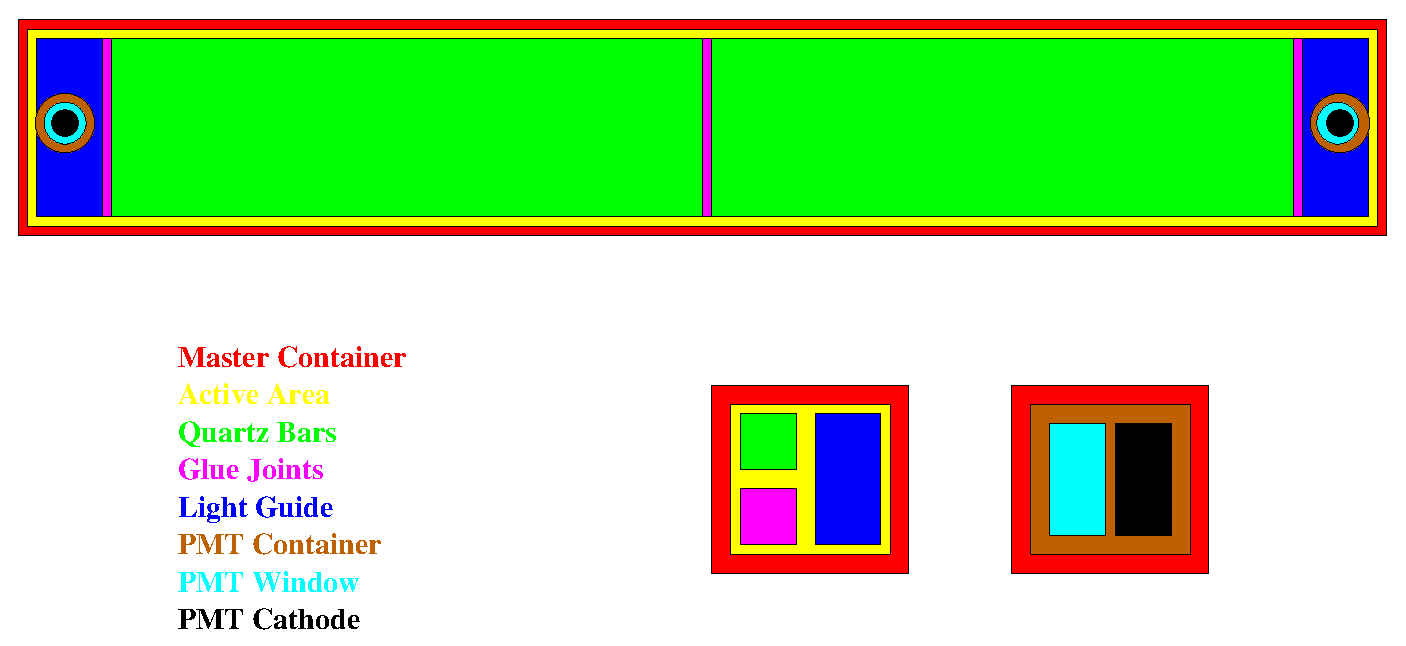
\includegraphics[scale=0.6]{./figures5/VolumeCont.eps}
  \caption{Volumes that make up the detector implentation and their
           containment within and with respect to each other. The
           detector active volume combines the quartz bars, the glue
           joints, and the light guides. The active area and the PMT
           container are contained within the master container, the
           PMT window and cathode, as well as an additional glue joint
           (not shown) are contained within the PMT container. Also
           not shown are several volumes used to simulate mirrored 
           surfaces.}
           \label{fig:VOLCONT}
\end{figure}

\subsubsection{Active Volume}

The active volume ({\it ActiveArea\_Physical}) is placed inside the
logical master container (lines 217 - 239, pp.~\pageref{SourceV4}) and
combines the volumes of the 2 quartz bars, three glue joints, one
between the bar and two at the ends, interfacing to the light guides
and the light guides themselves. The active volume's size is exactly
that of these 5 volumes combined and is specified as the sensitive
volume (lines 1181-1187, p.~\pageref{SourceV19}), for which hits are 
collected. The active volume material is air and as such, there is 
no distinction between this volume and the master container or the
mother volume (the experimental hall); it simply serves as a hit 
counter. Valid events are established when a particle generates
optical photons in the quartz bars or light guides. The corresonding
energy deposition and optical photon count for each event are collected
in the class {\it QweakSimSteppingAction} (chapter \ref{CHP_XVI}).
The active volume is also used to define the logical border surface for
the detector wrapping with various materials (millipore in this case)
(lines 1143 - 1172, pp.~\pageref{SourceV18}~-~\pageref{SourceV19}).
The active volume is specified as wrapped with millipore paper (lines
1150 - 1169, p.~\pageref{SourceV17}). This simulates the wrapping of
the quartz bars with some air between the bars and wrapping material.

\begin{table}
\begin{center}
\begin{tabular}{lll}
\hline 
 {\bf Property}          &  {\bf Detail}                     & {\bf Class}  \\
\hline 
 Geoemtry                &  13 main components for each      &  CerenkovDetector\\
                         &  octant including: 2 quartz bars, &  \\
                         &  2 light guides, 5 glue joints,   &  \\
                         &  2 cathodes, and 2 PMT entrance   &  \\
                         &  windows                          &  \\
                         &                                   &  \\ 
 Optical                 &  -refelectivity as a function     &  CerenkovDetector\\
 transport               &   of photon energy                &  Material\\ 
                         &  -absorption as a function of     &  UserInformation\\
                         &   energy                          &  EventAction\\
                         &  -index of refraction as a        &  \\
                         &   function of energy              &  \\
                         &  -cathode quantum efficiency      &  \\
                         &  -dielectric to dielectric        &  \\
                         &   boundary properties             &  \\
                         &                                   &  \\
 Sensitive               &  The quartz bars and PMT cathodes &  Cerenkov\_CerenkovSD    \\
 Volumes                 &  are both implemented as sensitive&  CerenkovDetector\_PMTSD \\
                         &   volumes.                        &  \\
                         &                                   &  \\
 Cuts and                &  -$\gamma$ \& x-ray energy cuts   &  CerenkovDetector        \\
 Event Readout           &  -particle definition and energy  &  Cerenkov\_CerenkovSD    \\
                         &   storage at time of hit          &  CerenkovDetector\_PMTSD \\
                         &  -secondary particle origin and   &  SteppingAction          \\
                         &   creator process                 &  \\
                         &  -quartz energy deposition        &  \\
                         &  -optical photon count            &  \\
\hline
\end{tabular}
\end{center}
\caption{List of detector properties that are currently implemented and 
         the corresponding classes where the code can be found.}
\label{tbl:V-II}
\end{table}

\subsubsection{Quartz Bars}

Lines 247 through 510 of the source code
(pp.~\pageref{SourceV4}~-~\pageref{SourceV8}) implement the quartz
radiator, consisting of two separate meter long quartz bars and three
glue joints. The material properties for the quartz are specified in
the class {\it QweakSimMaterial} (chapter~\ref{CHP_XVII}, lines 320 -
326, p.~\pageref{SourceXVII6}). The quartz bars are defined with
chamfers that can be adjusted for scew, which is the degree to which
they are not perfectly parallel with the edge of the quartz bar. This
amounts to a rotation around Z and Y, while the quartz bars are
oriented with their long axis along X. THis is done for all four long
edges of each meter long bar. Currently, for lack of complete knowledge
about the chemical composition, the glue joints are implemented
with the same material properties as the quartz bars. However, the 
actual glue joints used in the detector construction are made from a
silicon elastomere, so this should be good first order approximation.

\subsubsection{Light Guides}

Lines 512 through 704 (pp.~\pageref{SourceV9} - ~\pageref{SourceV11})
implement the light guide geometry. The guides are also made of quartz
and are chamfered as well. However, chamfer scew is not currently
implemented for the light guides. Although the light guide design is
now fixed to be rectangular, the guides are implemented here as
trapeziods (with the dimensions set to form a rectangle), because they
were adjusted to have various trpeziodal shapes during the design
process. The sculpting of the guide edges is also implemented so that
the left-right edges of the detector assembly can be cut at angles.
None of the guide sculpting is currently used (see lines 515 and 536),
leaving plain rectangular guides with 90 degree chamfered edges
everywhere. The mirroring of the guide faces and edges is implemented
between line 706 (p.~\pageref{SourceV12}) and line 800 (p.~\pageref{SourceV13}).
The face mirrors are currently turned off. The mirror material and 
optical properties are defined in the class {\it QweakSimMaterial}
(lines 363 - 370, p~\pageref{SourceXVII7}, 
lines 800 - 818, p.~\pageref{SourceXVII14}). 

\subsubsection{Pre (Shower) Radiator}

The implementation of the pre-radiator (lines 806 - 828,
p.~\pageref{SourceV13}) consists of a lead or tungsten bar placed in
fornt of the quartz (this is currently turned off).

\subsubsection{PMT Geometry}

Lines 833 (p.~\pageref{SourceV14}) through 993
(p.~\pageref{SourceV16}) implement the PMT, consisting of (in order,
as seen by a photon coming from the detector and traversing the PMT)
an entrance window, a glue layer, and a cathode (see
figs.~\ref{fig:PMTGEO} and ~\ref{fig:PMTGEO2}), all of which are
enclosed in the PMT container volume.  The thickness of the PMT
entrance window and cathode are rather arbitrarily set to be $1 {~\rm
mm}$. However, both volumes are typically much thinner in reality and
any simulated absorption in the window would therefore produce a lower
value in the simulated number of photons hitting the cathode, than
what would be expected on these grounds in the actual PMT. Lines 836
through 839 define variables needed to change the PMT position when
the light guides are changed to arbitrary trapezoids. Since the light
guides are now fixed to be rectangular, these variables are no longer
used.

\begin{figure}[h]
  \hspace{2cm}
  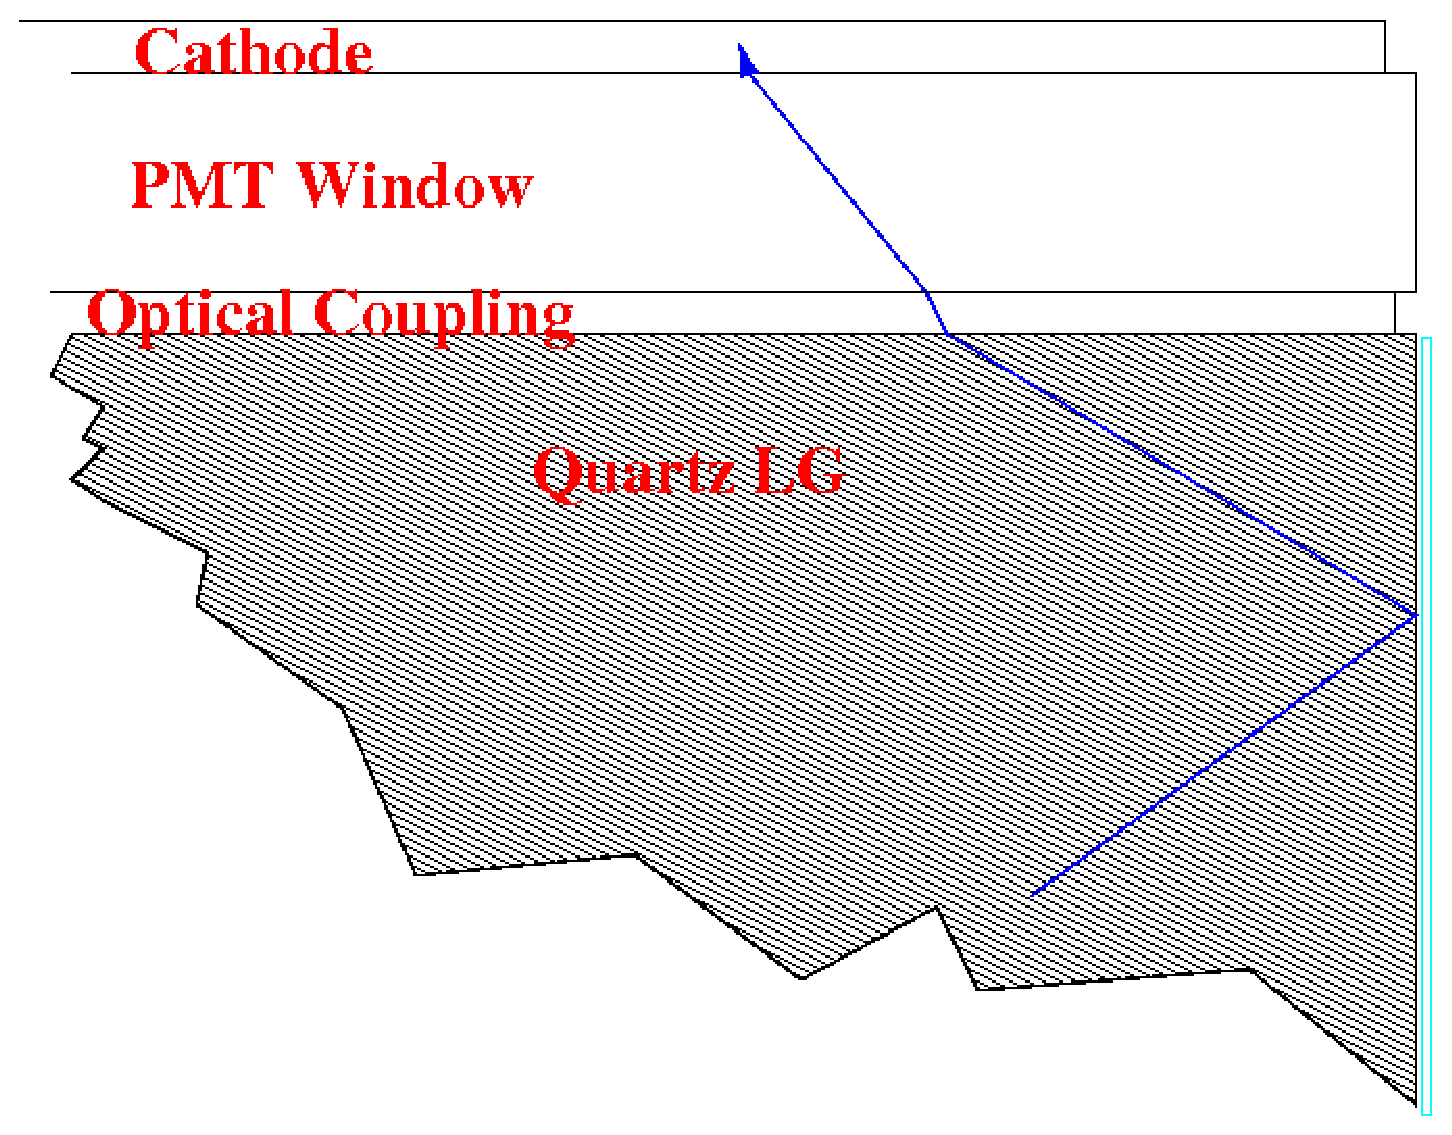
\includegraphics[scale=0.4]{./figures5/LightCountGeom.eps}
  \caption{Illustration of the PMT geometry and a photon ray through it.
           The right side of the light guide is shown as mirrored.}\label{fig:PMTGEO}
\end{figure}

\begin{figure}[h]
  \hspace{3cm}
  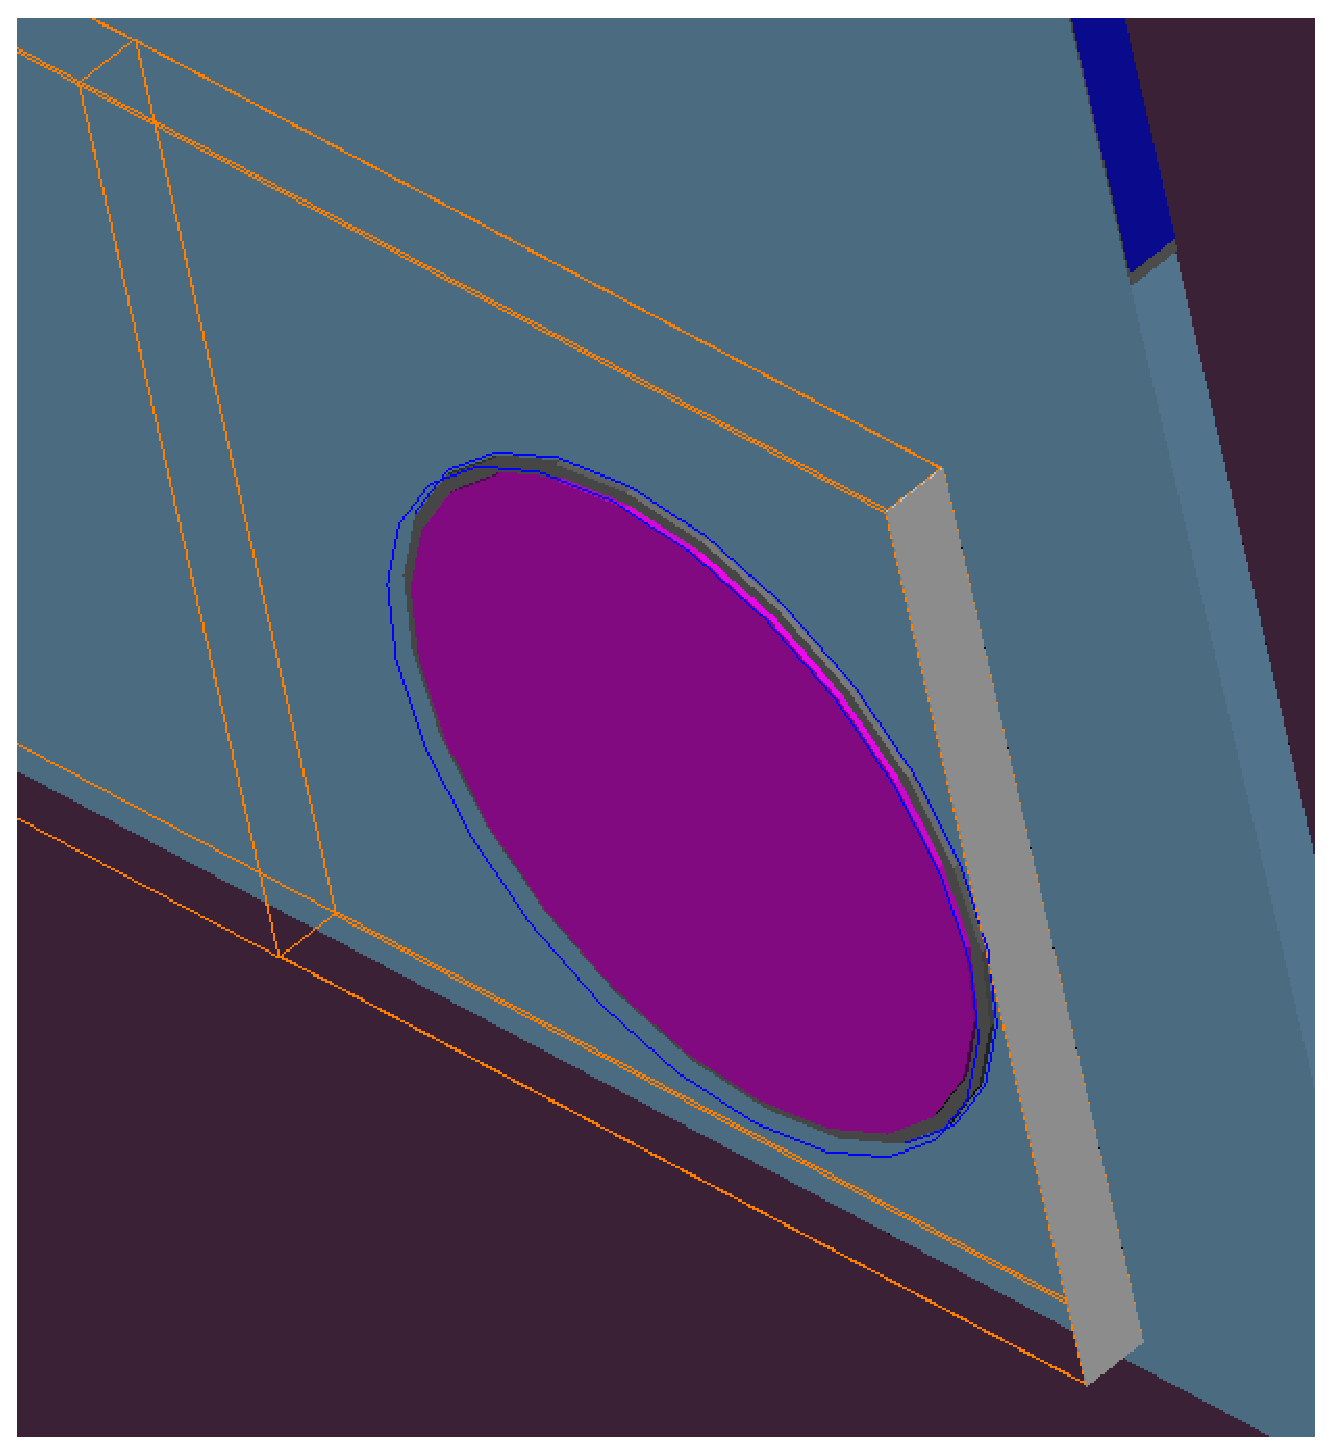
\includegraphics[scale=0.4]{./figures5/PMTGeometry.eps}
  \caption{PMT geometry in the simulation, with an entrance window (grey),
           a cathode (magenta), and the container (blue wire frame). The
           glue joint is not visible.}\label{fig:PMTGEO2}
\end{figure}


\subsection{Optical and Related Properties}

The optical properties of the main detector are specified for the
quartz bars, the light guides, the PMT cathode and entrance windows,
all glue joints, and a wrapping layer around the active volume.  The
implemented optical properties include wavelength dependent index of
refraction, absorption coefficient (length), reflectivity as well as
surface properties (roughness, interface type, etc..). Most of these
are specified in the {\it QweakSimCerenkovDetector} and {\it
QweakSimMaterial}. The only exception is the quantum efficiency of the
S20 cathode used in the experiment (fig.~\ref{fig:PMTQE}), which is
specified in {\it QweakSimUserInformation} (lines 54,
p.~\pageref{SourceXVIII3} through 154, p.~\pageref{SourceXVIII5}).

\subsubsection{Quartz}

The emission wavelength range for the quartz bars is 250 to 800 nm,
but sharply peaked around 280 nm. Based on that, the optical
properties are specified for wavelengths for 210 to 800 nm
wavelengths.  The optical properties for the quartz (including the
light guides)(except for the reflectivity) are specified in the class
{\it QweakSimMaterial}, (chapter~\ref{CHP_XVII}, lines 708 - 758,
pp.~\pageref{SourceXVII12}-~\pageref{SourceXVII13}).  The reflectivity
is implemented in the detector source file itself (lines 1030-1057,
p.~\pageref{SourceV17} and line 1135, p.~\pageref{SourceV18}),
together with the surface definitions, since it is a surface property
rather than a bulk material property.  The surface polish specified to
the bar manufacturer is 25 Angstroms~\cite{tn:MACK1} with an average
reflectivity of 0.997. The specified reflectivity follows an emperical
equation (eqn.~\ref{eqn:qrefl})~\cite{tn:NEVEN}.
\begin{equation}
  R = 1-0.027e^{-0.0046\lambda}~.\label{eqn:qrefl}
\end{equation}

Lines 1059 through 1140 define the border surfaces between the quartz
bar and the active volume, including the surface roughness (polish),
the interface type (dielectric to dielectric) and the model (glisur,
see section~\ref{G4OPTR}).

\subsubsection{PMT}

Since the real PMT windows are specifically UV transmitting, the
simulated window material has been set to quartz (i.e. a perfect index
of refraction match). However, the index of refraction for the glue
joints used here (and between the quartz bars and light guides
described above) is different from the one used for the quartz (see
class {\it QweakSimMaterial}, lines 767 - 777,
p.~\pageref{SourceXVII13}). Currently, there is only one value
available for the index of refraction of the glue~\cite{pc:MACK1}
which has been used over the wavelength range of interest. There is
currently also no information on hand for the absorption length of the
elastomere glue, which has therefore been set to be identical to that
of the quartz~\cite{tn:BABAR}. 

\begin{figure}[h]
  \hspace{0cm}
  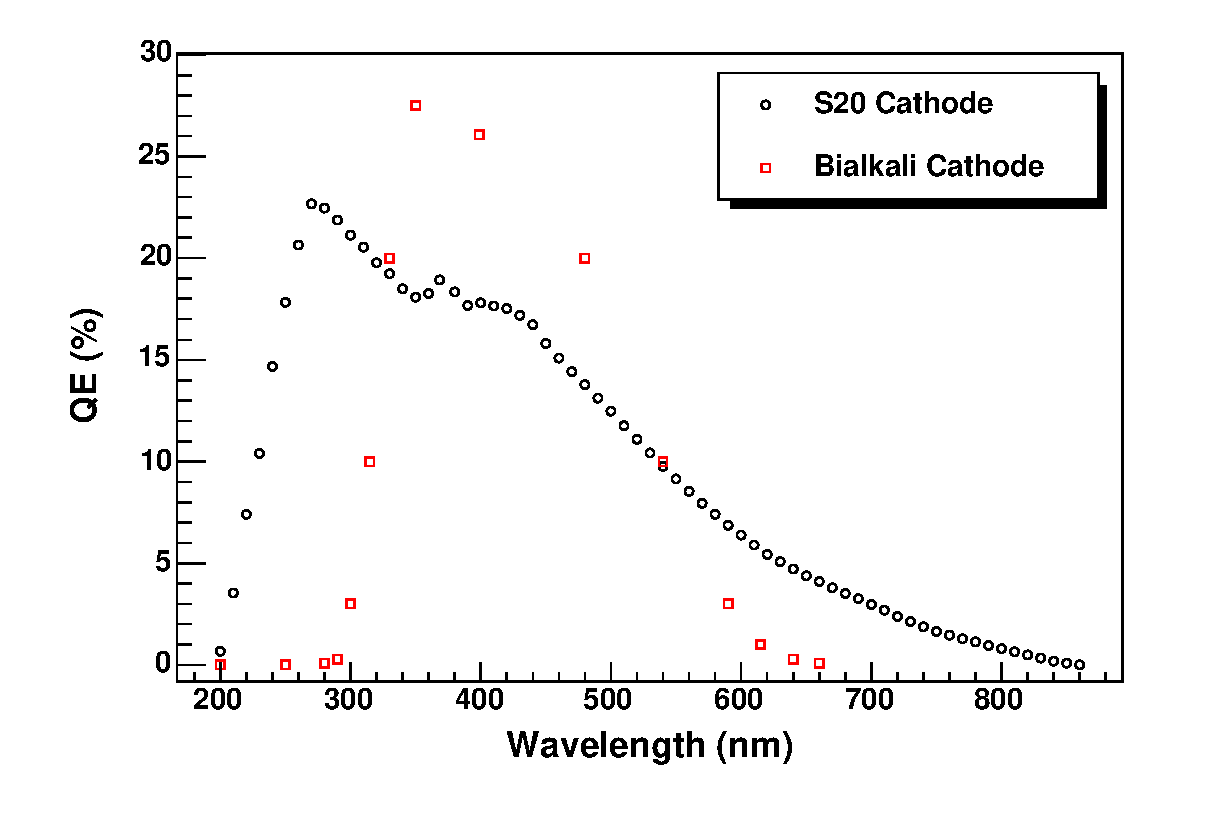
\includegraphics[scale=0.6]{./figures5/PMTCathQE.eps}
  \caption{Quantum efficiency for the S20 cathode PMT to be used in the
           experiment~\cite{PC:EELECTRONTUBES}.}
           \label{fig:PMTQE}
\end{figure}

\subsubsection{Detector Wrapping}

The millipore paper optical properties are specified in lines 1156
through 1160. The reflectivity is a measured quantity~\cite{PC:LLEE}
(fig.~\ref{fig:REFLECTANCE}) for part of our wavelength range. The
values for the remaining range are guessed, based on the assumption
that the trend of the curve continues uniformely beyond the plotted
range. The significance and meaning of the boundary interface models,
surface finish, and other settings are discussed in
section~\ref{G4OPTR}.  For some models, the specification of the
relative strengths of the type of light scattering is required. Lines
1156 through 1160 set the reflectivity of the wrapping material itself
and the strengths of 3 of the 4 scattering types, where the fourth is
Lambertian reflection, which is set by GEANT4 such that all four types
add up to 1. The actual relative strengths are often not known for
materials, so that, in this case, the values are guessed according to
what the material "looks" like. For millipore paper, the values for
backscatter and specular reflection are set to be 30\% compared to
70\% for lambertian or diffuse reflection, since the material is known
to have a rather dull appearance. It is assumed that all light is reflected
in some way or another and the absorption length for the wrapping material 
is currently not set (meaning that GEANT4 sets it to zero).


\begin{figure}[h]
  \hspace{0cm}
  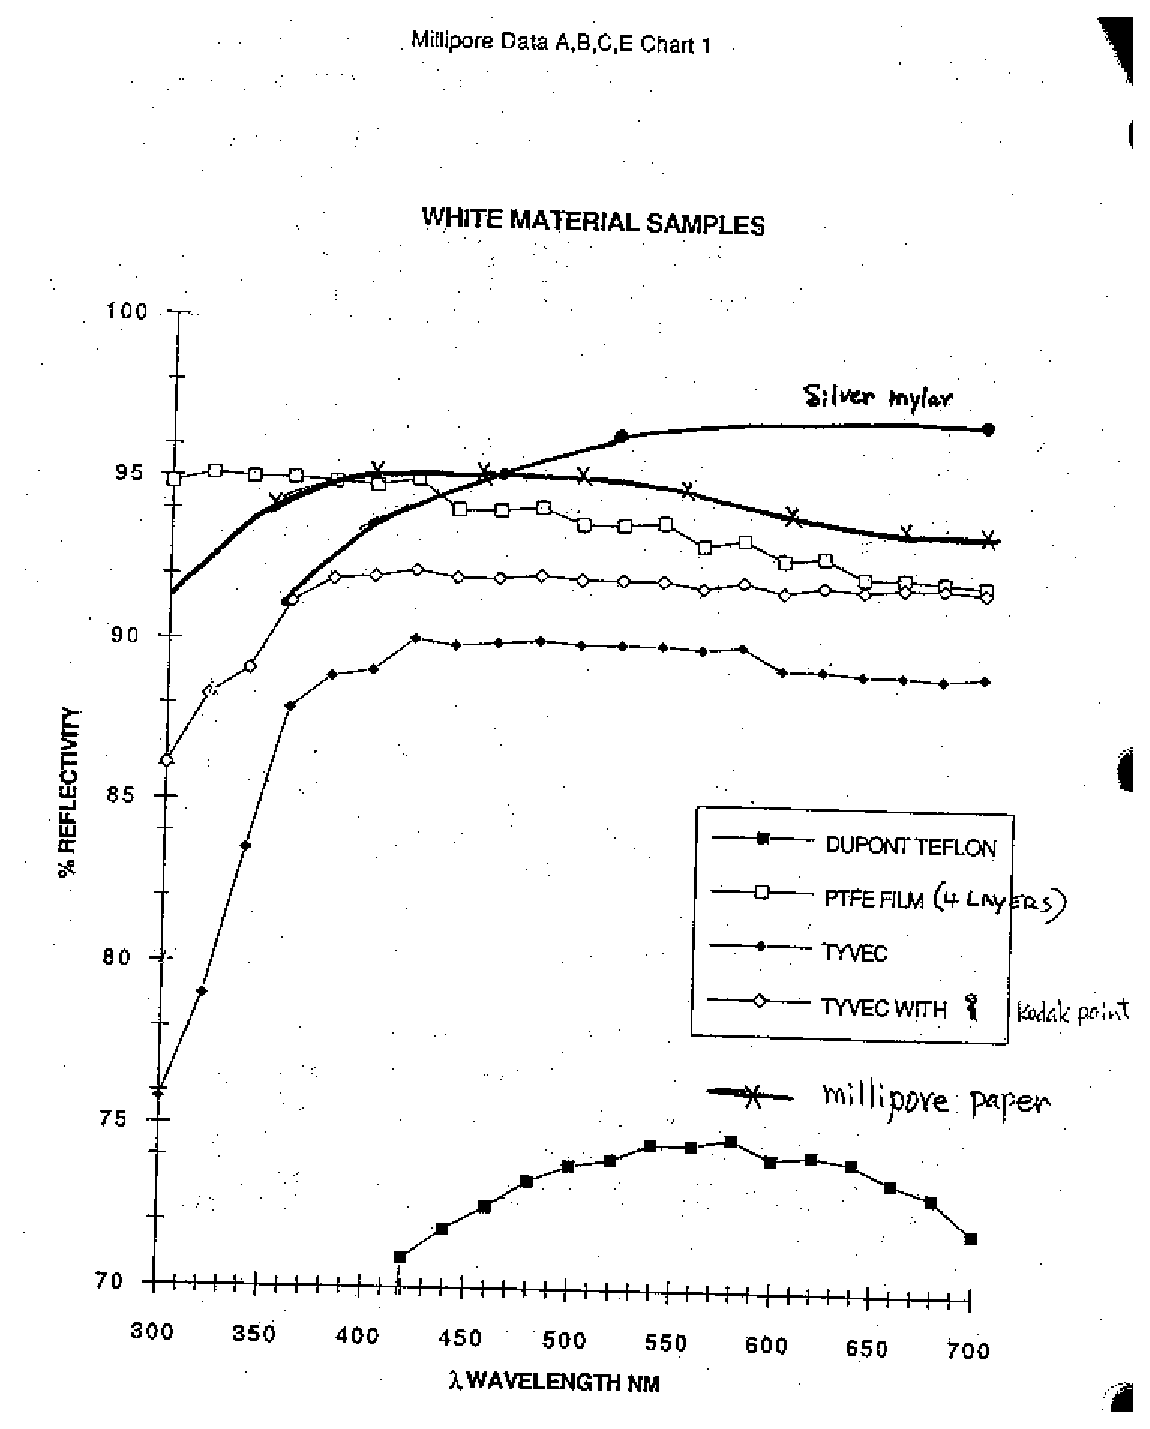
\includegraphics[scale=0.7]{./figures5/Wrapping-Material-Reflectance.eps}
  \caption{Reflectance of various detector wrapping materials~\cite{PC:LLEE}.}
           \label{fig:REFLECTANCE}
\end{figure}

\clearpage

\section{Description of the Geant4 Optical Transport and Transmission Code \\
         ({\it G4OpBoundaryProcess})}\label{G4OPTR}

The GEANT4 class {\it G4OpBoundaryProcess} handles reflection and
refraction at optical boundaries between two volumes, taking into
account the photon polarization. A detailed trace was done of this
class to benchmark the simulation and to be able to correctly
implement the optical properties described above, as well as to
correctly interpret the simulation output. The generation of Cerenkov
light and bulk absorption are handled in classes {\it G4Cerenkov} and
{\it G4OpAbsorption} respectivley. 

A GEANT4 event is split into tracks of the primary and possible
secondary particles. Each track is separated into steps, with each
individual step size being determined by a particular physics
interaction with the shortest associated range in a given
material. Please consult the GEANT4 manuals for more
information~\cite{tn:GEANT4SFM}.  A step in GEANT4 is defined by its
two end points {\em preStepPoint} and {\em postStepPoint}.  All registered
continuous and discrete processes are called for each step. The class
{\it G4OpBoundaryProcess} implements a discrete process and these are
handled by the stepping manager class after the step is completed, by
calling tha function {\it PostStepDoIt} in the {\it G4OpBoundaryProcess}
class.

\subsection{Function {\it PostStepDoIt}}
The function begins by checking whether the photon is traversing a
boundary ({\em postStepPoint} lies in the next volume) and if the step
size would be large enough to actually push the photon into the next
volume and returns without doing anything if either condition is not
met (fig.~\ref{fig:OPBOUND1}).

\begin{figure}[h]
  \hspace{3cm}
  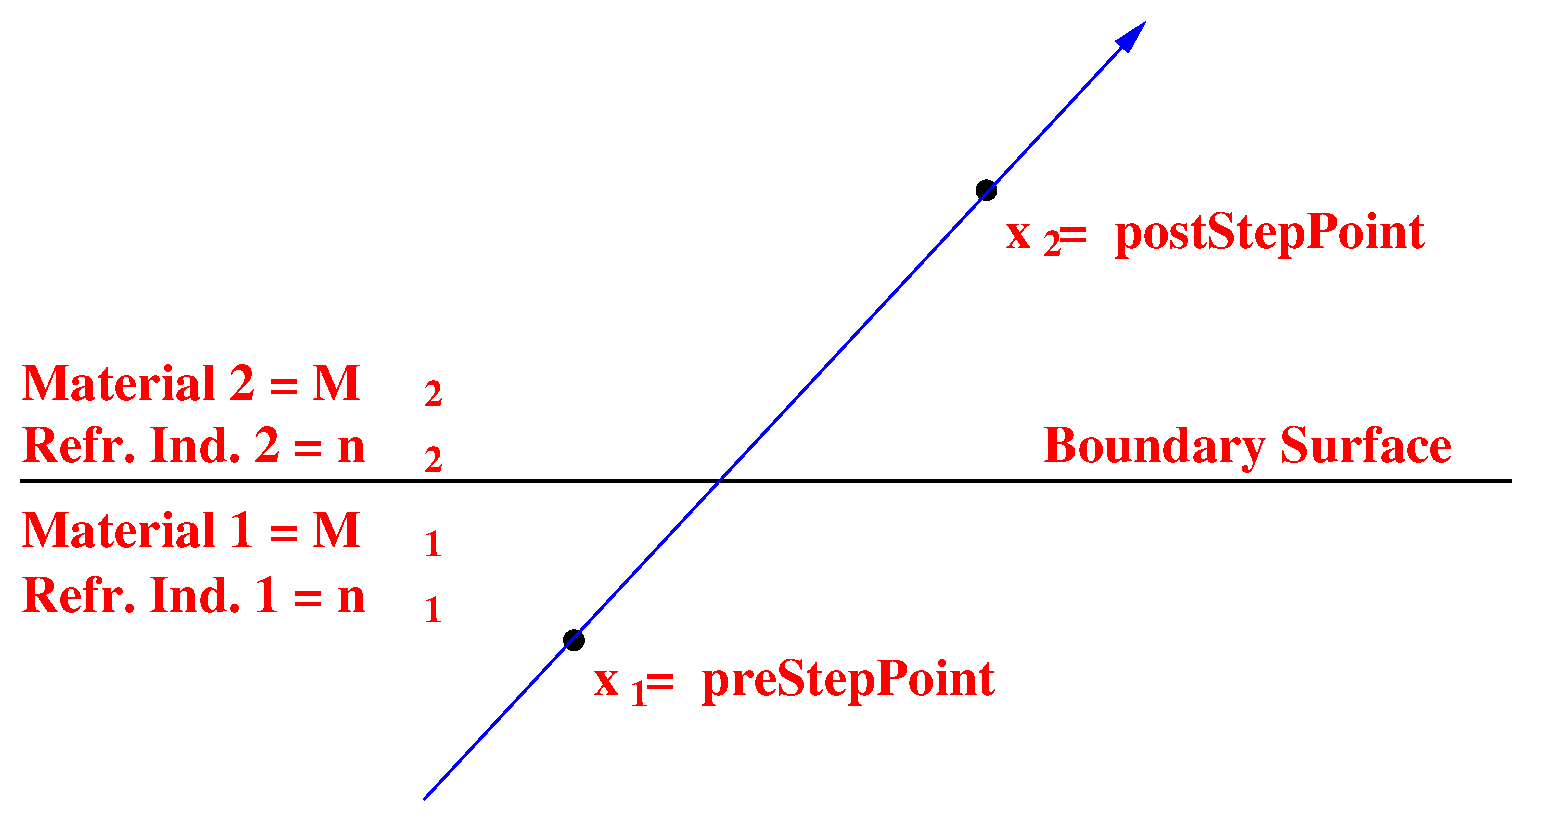
\includegraphics[scale=0.4]{./figures5/OpBoundary01.eps}
  \caption{Illustration of optical boundary variables.}
           \label{fig:OPBOUND1}
\end{figure}

The variables for the material definitions $(M_1,~M_2)$, indicies of
refraction $(n_1,n_2)$, old (before the boundary process is invoked)
photon momentum $(|\vec{k}_1| \equiv k_1)$, direction $(\hat{k}_1)$
and polarization $(\hat{h}_1)$ are obtained. The index of
refraction in material 1 $(n_1)$ is obtained according to the momentum
of the incident photon. For Cerenkov light, the photon momentum and
polarization is determined in the class {\em G4Cerenkov}.

If the electron momentum direction is taken to lie along the the
positve Z axis then the photon momentum lies along a cone with opening
angle $(\theta)$ such that $$\sin^2\theta \leq \sin^2\theta_{max},$$
with $$\cos\theta = \frac{1}{\beta n(f)}$$ and $\sin\theta_{max}$ is
set by $\cos\theta_{max} = 1/\beta/n(f_{max})$, where $f_{max}$ is the
maximum user specified index of refraction, corresponding to the
maximum user specified photon momentum (see class {\it
QweakSimMaterial}, chapter~\ref{CHP_XVII}, lines 708 - 758,
pp.~\pageref{SourceXVII12}-~\pageref{SourceXVII13}).  In a general
right handed coordinate system, the photon momentum is then simply set
to
\begin{eqnarray}
\hat{k_x} &=& \sin\theta\cos\phi \nonumber \\ 
\hat{k_y} &=& \sin\theta\sin\phi \nonumber \\ 
\hat{k_x} &=& \cos\theta~. \nonumber \\ \nonumber 
\end{eqnarray}
The photon polarization is set to be linear and orthogonal to the
momentum direction, in accordance with the property of transverse 
polarization in electromagnetic waves (fig.~\ref{fig:OPBOUND2}). 
\begin{eqnarray}
\hat{h_x} &=& \cos\theta\cos\phi \nonumber \\ 
\hat{h_y} &=& \cos\theta\sin\phi \nonumber \\ 
\hat{h_x} &=& -\sin\theta \nonumber \\ \nonumber 
\end{eqnarray}
\begin{figure}[h]
  \hspace{4cm}
  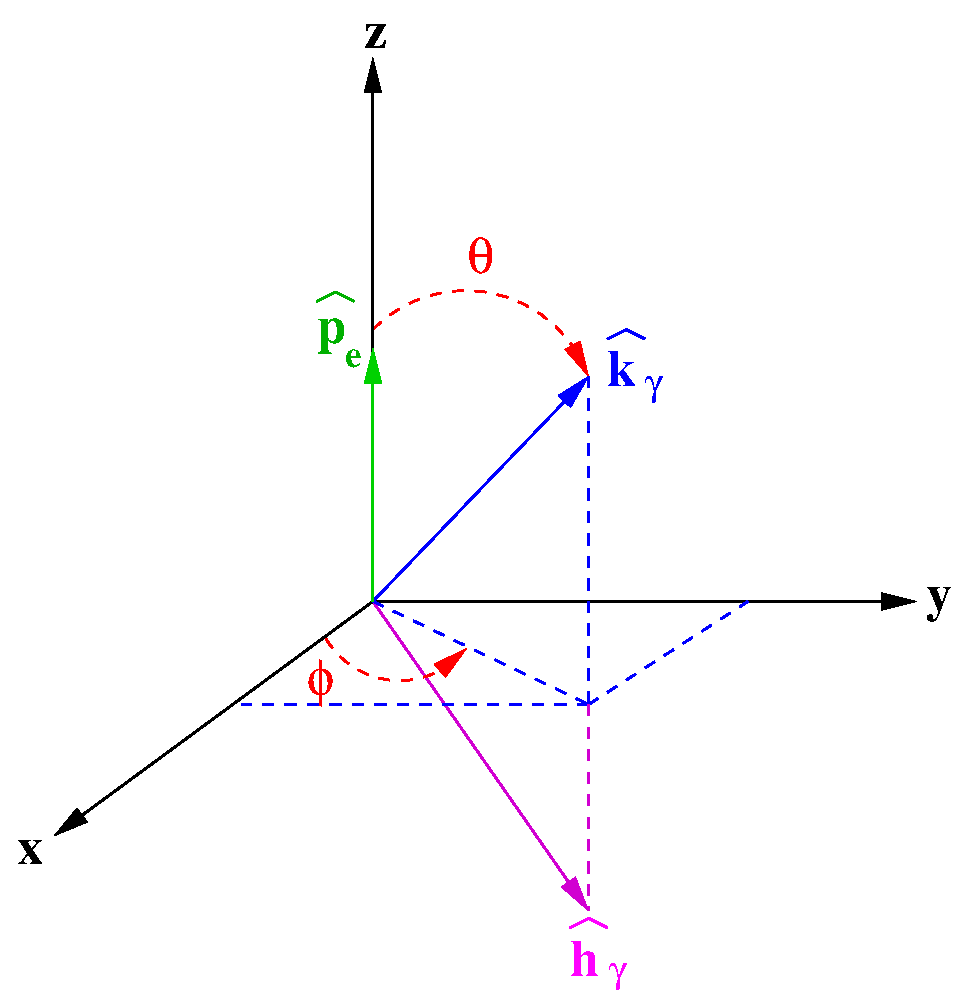
\includegraphics[scale=0.3]{./figures5/OpBoundary02.eps}
  \caption{Cerenkov photon momentum and polarization with respect to 
           the direction of an incident electron, in Geant4.}
           \label{fig:OPBOUND2}
\end{figure}
The azimuthal angle is chosen randomly from a uniform distribution,
between $0$ and $2\pi$.

Next, a pointer to the logical border surface $(s_1)$ between the two
volumes containing $x_1$ and $x_2$ is obtained. This is one of the
surfaces specified in class {\em QweakSimCerenkovDetector} (lines 1071
through 1095, pp.~\pageref{SourceV17},~\pageref{SourceV18} and line
1147, p.~\pageref{SourceV19}). From this in turn, the optical surface
properties are obtained, providing access to the interface type
(dielectric-dielectric, dielectric-metal, etc..), the physics
treatment model (glisur or unified~\cite{pp:LEVMOI}, see below), and
the surface finish (polished, ground, {\em backpainted}, {\em
frontpainted}, see below).  The optical surface object also provides
access to the material properties as specified on lines 1135 through
1142 (p.~\pageref{SourceV18}) and lines 1165 through 1175
(p.~\pageref{SourceV19}).


If the model is glisur, only the reflectivity and efficiency (for
absorption at the surface, which is not to be confused with the bulk
absorption length of the material, set in the class {\it
QweakSimMaterial}, see above) are accessed according to the photon
momentum. If they are not specified, then the reflectivity is set to
unity and the absorption efficiency is set to zero. The surface
absorption efficiency of the quartz is not currently set. If the model
is unified, then, in addition to the efficiency and absorption, the
particular scattering properties (see section on wrapping above) are
accessed as well. If any of the specular reflection types or
backscatter are not specified, they are set to zero, which
automatically makes all scattering maximally diffuse (lambertian). 

In the case of use of the glisur model and if the finish is polished
or ground and the interface is between two dielectric materials, the
simulation attempts to get the index of refraction of material two
$(n_2)$ from the surface material properties table. This is done
unless material one is identical to material two, in which case no
further action is taken (the photon is returned to the stepping
manager). If the finish is ground or polished {\em backpainted}
(smooth and rough wrapping respectively, using the unified model --
don't blame me, didn't make up those names), the simulation attempts
to get the index of refraction of the layer between the surface and
the wrapping.

\begin{verbatim}
NOTE: If the surface material properties table is not given for a
      specified optical surface, and the surface finish is
      polishedbackpainted or groundbackpainted, then GEANT4
      kills the track. I.e. the photon is lost at the boundary.

      The same is true for polished or ground glisur model surface
      specifications if no index of refraction was specified for
      material two. 
\end{verbatim}

Lines 1100 through 1133 (p.~\pageref{SourceV18}) use the glisur model
with a polished surface finish requiring the specification of a polish
level for the quartz. This surface interface is illustrated in
fig.~\ref{fig:OPBOUND1}. Lines 1152 through 1165
(p.~\pageref{SourceV19}) implement the detector wrapping and use the
unified model with a {\em groundbackpainted} finish, including the
specification of all scattering parameters and the wrapping material
roughness parameter $(\sigma_{\alpha})$.  This setup is illustrated in
fig.~\ref{fig:OPBOUND3}. If the finish is specified to be {\em
frontpainted} the configuration corresponds to that in
fig.~\ref{fig:OPBOUND3}, but without the layer between the optical
surface and the wrapping; this then corresponds to more of a coating
rather than a wrapping. 

Still in the function {\em PostStepDoIt}, the simulation then obtains
the global position $(\vec{x}_g)$ of the photon, as given by the {\em
postStepPoint} (see fig.~\ref{fig:OPBOUND1}).  The global position
vector is then transformed to the local volume coordinate system
$\vec{x}_l = {\bf T} \vec{x}_g$. The reverse is done for the vector
normal to the volume surface which the photon is hitting
$(\hat{n}_l)$, which is given in the local volume coordinate
system. The local normal points away from the volume and the negative
$(\hat{n}^{'}_l \equiv -\hat{n}_l)$ of this vector is transformed to
the global coordinate system $\hat{n}_g = {\bf T}^{-1}\hat{n}^{'}_l$.
The transformation matrix $({\bf T})$ transforms around the local
normal $(\hat{n}^{'}_l)$. These transformations are necessary since
all Geant4 particle momenta are specified in global coordinates.

\begin{figure}[h]
  \hspace{4cm}
  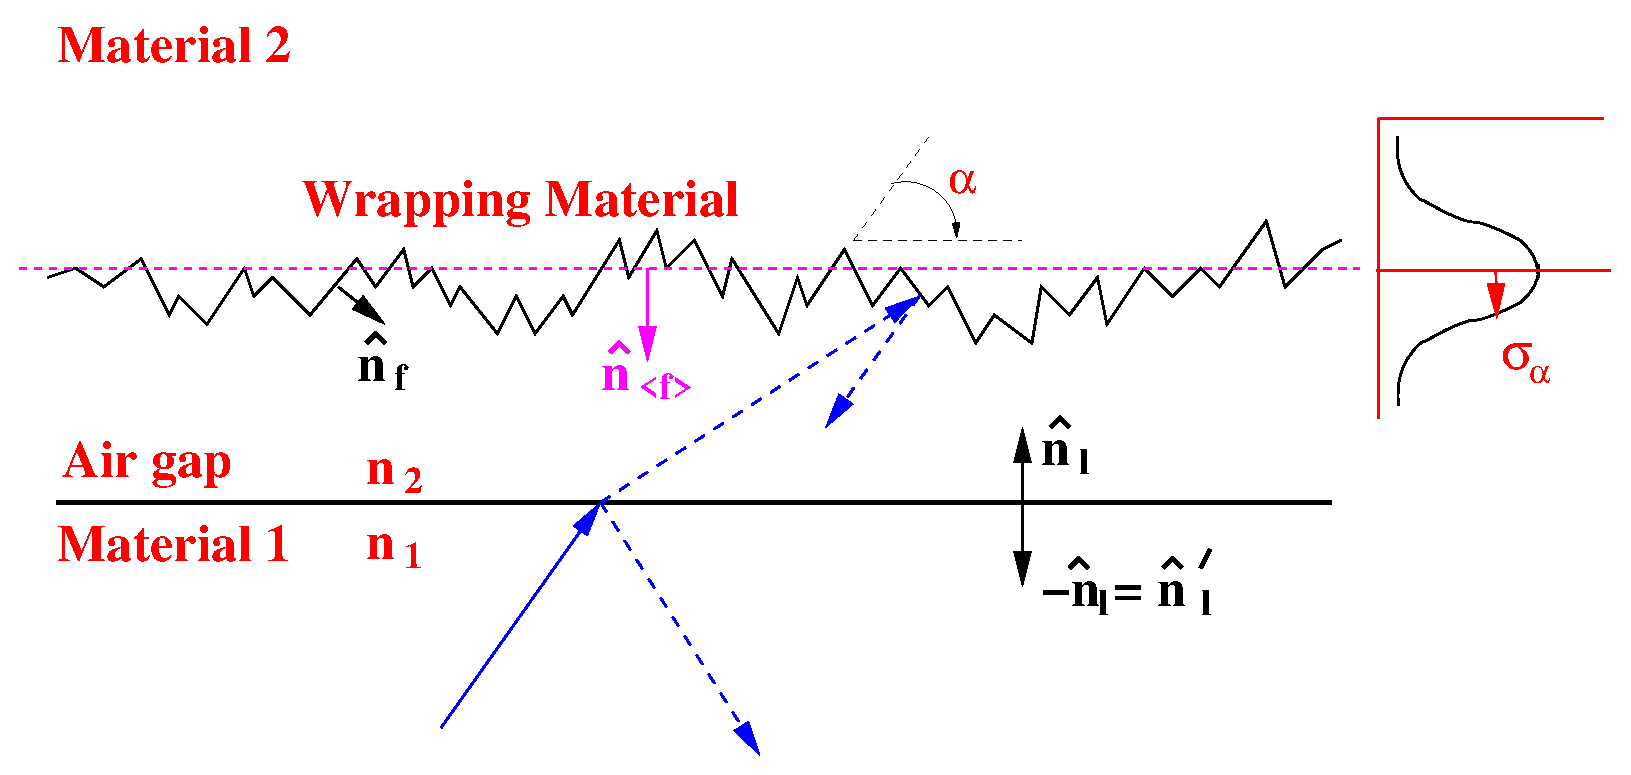
\includegraphics[scale=0.3]{./figures5/WrappingFig.eps}
  \caption{Illustration of the material index of refraction for
           a wrapped detector configuration, inlcuding specification
           of the wrapping material roughness.}
           \label{fig:OPBOUND3}
\end{figure}

Next, the simulation checks ot make sure that $\hat{k}_1 \cdot
\hat{n}_g \leq 0$, and otherwise forces this to be the case by setting
$\hat{n}_g \Rightarrow -\hat{n}_g$.  Then, if the interface type is
dielectric-metal, the function {\em DielectricMetal} is called. If the
interface type is dielectric-dielectric and the surface finish is {\em
frontpainted} (coating) then it is randomly determined of the photon
is absorbed or reflected. This is done by uniformly sampling a random
variable between zero and one and choosing reflection if the random
variable is less than the specified reflectivity and choosing
absorption otherwise (See the function {\em G4BooleanRand} in the {\em
G4OpBoundaryProcess} header file). If the photon is reflected and the
finish is {\em groundfrontpainted} (a rough coating) then the
reflection is lambertian. If the interface is dielectric-dielectric
and the finish is anything other than {\em frontpainted } then the
function {\em DielectricDielectric} is called. This is the case we
concentrate on here. This function handles the details of reflection,
transmission/refraction and absorption at the boundary between two
dielectric materials, and includes the implementation of wrapping
or coating.

\subsection{Function {\em DielectricDielectric}}

The function {\em DielectricDielectric} consists of two nested loops
that are cycled through as long as the photon has either not made a 
transmission from the origin volume to another volume nor a 
valid reflection back into the same volume (inner loop), or as long 
as the photon continues to be reflected from the wrapping (or the surface
of the volume the photon is transmitted to) (outer loop).

The function begins by comupting the so called facet normal
$\hat{n}_f$ (see fig.~\ref{fig:OPBOUND3}) if the surface finish is
{\em ground} or {\em groundbackpainted}. Otherwise the facet normal
is set to be equal to the global normal $\hat{n}_g \equiv \hat{n}_{\expec{f}}$,
which is assumed to be parallel with the surface normal of volume 1,
containing the incident photon. The facet normal can either correspond
to the normal of a small area on the wrapping  material or to the 
normal of a facet on the rough surface of volume 1.

The facet normal is obtained as follows:

If the surface model is not unified (i.e. glisur) then the function
obtains the polish of the volume 1 surface (note the volumes 1 and 2
pointers passed to the {\em G4LogicalBorderSurface} constructor
starting on line 1071 p.~\pageref{SourceV17}). If the polish is 1
(100\%) then the facet normal is set to be equal to the global normal
$(\hat{n}_f = \hat{n}_g)$. If the polish smaller than 1, then the 
following procedure is used to randomly find the facet normal:

\begin{enumerate}
  \item{establish a vector $\vec{s}$, such that
    \begin{enumerate}
      \item{$-1 \leq s_x \leq 1$ randomly chosen with uniform distribution}
      \item{$-1 \leq s_y \leq 1$ randomly chosen with uniform distribution}
      \item{$-1 \leq s_z \leq 1$ randomly chosen with uniform distribution \\
            \\
            with the condition that $|\vec{s}| \leq 1$}
    \end{enumerate}
  } 
  \item{set $\vec{s} = (1-{\rm Polish})\vec{s}$}
  \item{set $\vec{n}_f = \hat{n}_g + \vec{s}$}
  \item{repeat this process until $\vec{k}_1 \cdot \vec{n}_f < 0$}
  \item{renormalize $\vec{n}_f \Rightarrow \hat{n}_f$}
\end{enumerate}

If the model is unified, the following procedure is used:

\begin{enumerate}
  \item{The process obtains $\sigma_\alpha$ from the optical
        surface. \\ This parameter specifies the surface roughness of
        the reflector (wrapping). See fig~\ref{fig:OPBOUND3}. $\alpha$
        is the angle a facet surface makes with respect to the average
        surface.  $\alpha$ is randomly choosen repeatedly, from a
        gaussian distribution with standard deviation $\sigma_\alpha$,
        until the following conditions are met:
    \begin{enumerate}
      \item{$f_m \times r \leq \sin\alpha$ or $\alpha < \pi/2$, \\ 
            where $r$ is a random variable between 0 and 1, with 
            uniform distribution and,}
      \item{$f_m = 4\sigma_\alpha$ as long as $4\sigma_\alpha < 1.0$
            and $f_m = 1.0$ otherwise.}
    \end{enumerate}
  }
  \item{A unit vector $(\hat{u})$ is established from \\
        $u_x = \sin\alpha \cos\phi$ \\
        $u_y = \sin\alpha \sin\phi$ \\
        $u_z = \cos\alpha$ \\
        where phi is randomly chosen between $0$ and $2\pi$, with uniform
        distribution.}
  \item{$\hat{n}_f \equiv \hat{u}$}
  \item{this process is repeated until $\vec{k}_1 \cdot \vec{n}_f < 0$}
\end{enumerate}

The simulation then determines whether the photon undergoes total internal
reflection, refraction or is absorbed at the boundary. The program calculates

\begin{eqnarray}
  \hat{k}_1 \cdot \hat{n}_f &=& \cos\theta_{k_1} ~~~{\rm (Note~that~this~is~negative)} \nonumber \\
  \hat{h}_1 \cdot \hat{n}_f &=& \cos\theta_{h_1} \nonumber \\ \nonumber
\end{eqnarray}

If the incident angle is oblique $(-\cos\theta_{k_1} < 1.0)$, the simulation
code calculates the outgoing photon angle (fig.~\ref{fig:OPBOUND4})
$$\sin\theta_{k_2} = \frac{n_1}{n_2}\sin\theta_{k_1}$$ in the standard
way, according to Snell's Law. Note that, if the surface finish was
specified to be {\em backpainted}, then $n_2$ is the index of
refraction for the material layer between volume 1 and the wrapping
(see fig.~\ref{fig:OPBOUND3}). If the photon is normally incident
$(-\cos\theta_{k_1} \geq 1.0)$ the simulation sets $\sin\theta_{k_1} =
\sin\theta_{k_2} = 0$.

\begin{figure}[h]
  \hspace{4cm}
  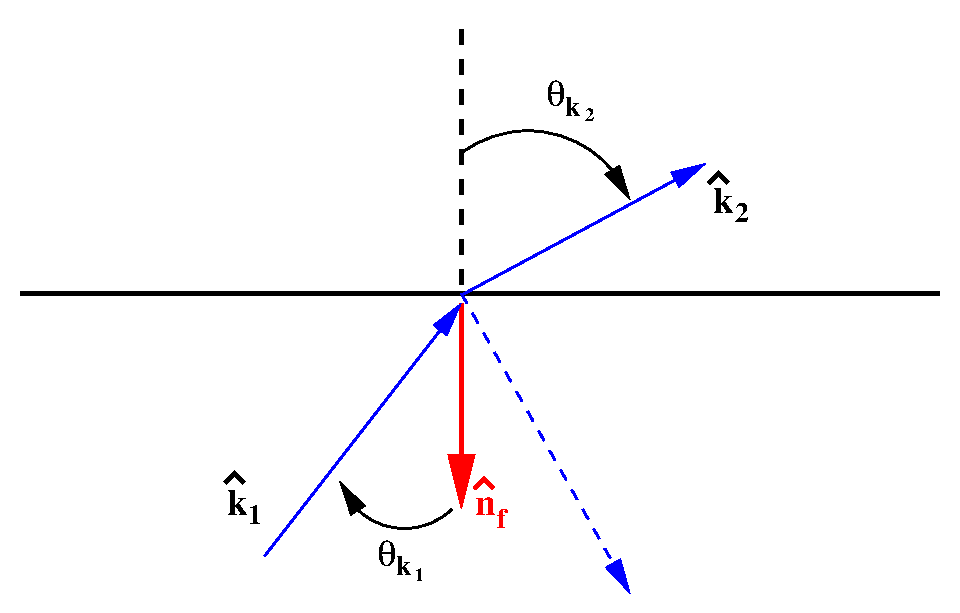
\includegraphics[scale=0.3]{./figures5/OpBoundary03.eps}
  \caption{Illustration of standard reflection and refraction at 
           the boundary and the variables used here.}
           \label{fig:OPBOUND4}
\end{figure}

The program continues to go through the simulation for total internal
reflection if $\sin\theta_{k_2} \geq 1$ and otherwise goes on to
simulate transmission/refraction and reflection, including
polarization.

\subsubsection{Total Internal Reflection}

For total internal reflection, if the model is unified and the finish
is not polished, the program determines a specific reflection type
from the photon wavelength dependend parameters, specified by the
user, specular spike $(\rho_{ss})$, specular lobe $(\rho_{sl})$,
backscatter $(\rho_{bs})$. Together with the parameter for lambertian
reflection, which is set automatically, these parameters have to add
to unity. A uniformely distributed random variable $(r)$ is then
sampled between 0 and 1, and the reflection type is determined as

\begin{enumerate}
  \item{specular spike reflection if: $0 \leq r < \rho_{ss}$ (In this case $\hat{n}_f = \hat{n}_g$)}
  \item{specular lobe reflection if : $\rho_{ss} \leq r \leq \rho_{ss} + \rho_{sl}$}
  \item{backscatter if              : $\rho_{ss} + \rho_{sl} < r < \rho_{ss} + \rho_{sl} + \rho_{bs}$ and}
  \item{Lambertian reflection if    : $ \rho_{ss} + \rho_{sl} + \rho_{bs} \leq r \leq  1$~.}
\end{enumerate}

If the reflection is Lambertian (diffuse), a new momentum is randomly
chosen around the global normal $(\hat{n}_g)$, such that it lies in
the same hemisphere as the global normal. The facet normal is then
calculated from $\hat{n}_f = (\vec{k}_2 - \vec{k}_1)/(|\vec{k}_2 -
\vec{k}_1|)$ and the new polarization is calculated from $\hat{h}_2 =
-\hat{h}_1 + 2(\hat{h}_1\cdot\hat{n}_f)\hat{n}_f$.  This just sets
$\vec{E}_{new} = -\vec{E}_{old}$ $(\vec{E} \equiv \vec{h})$, making
sure that this happens around the facet normal and in the plane of
incidence. For total internal reflection, this satisfies the standard 
boundary conditions (see, for example,~\cite{bb:JACKSON,bb:HECHT})
\begin{eqnarray}
  \epsilon_1\left(E^{\perp}_{I} + E^{\perp}_{R}\right) &=& \epsilon_2 E^{\perp}_{T}  \nonumber \\
                             E^{\parallel}_{I} + E^{\parallel}_{R} &=& E^{\parallel}_{T}~. \nonumber \\ \nonumber
\end{eqnarray}

If the photon is backscattered, then $\hat{k}_2 = -\hat{k}_1$ and
$\hat{h}_2 = -\hat{h}_1$. If the photon is neither backscattered nor
Lambertian reflected (i.e. the reflection is specular lobe or specular
spike), then
\begin{eqnarray}
  \hat{k}_2 &=&  \hat{k}_1 - 2(\hat{k}_1\cdot\hat{n}_f)\hat{n}_f  \nonumber \\
  \hat{h}_2 &=& -\hat{h}_1 + 2(\hat{h}_1\cdot\hat{n}_f)\hat{n}_f~. \nonumber \\ \nonumber
\end{eqnarray}

For total internal reflection, the function {\em DielectricDielectric} then
exits with $\hat{k}_2\cdot\hat{n}_g \geq 0$ and $\hat{k}_1 = \hat{k}_2$,
$\hat{h}_1 = \hat{h}_2$, returning the new momentum and polarization after
the reflection to the stepping manager which continues to step the photon
through the volume, until it encounters another boundary or is killed by
some other process.

\subsubsection{Calculation of Transmission Amplitude}

Here, the simulation determines whether a photon is reflected or
transmitted, based on the size of the calculated transmission
coefficient.

If $\sin\theta_{k_2} < 1$, then the simulation calculates
\begin{eqnarray}
  \cos\theta_{k_2} &=&  \sqrt{1-\sin^2\theta_{k_2}} ~~~~~{\rm for}~\cos\theta_{k_1} > 0 \nonumber \\
  \cos\theta_{k_2} &=& -\sqrt{1-\sin^2\theta_{k_2}} ~~~~~{\rm for}~\cos\theta_{k_1} \leq 0 \nonumber \\ \nonumber
\end{eqnarray}
For oblique angles of incidence $(\sin\theta_{k_1} > 0)$, the parallel and
perpendicular components of polarization are calculated as follows.
\begin{enumerate}
  \item{Determine a unit vector perpendicular to the plane of incidence: \\
        $\hat{A}_{\perp} = \frac{\vec{k}_1\times\hat{n}_f}{|\vec{k}_1\times\hat{n}_f|}$\\
        If, in figure~\ref{fig:OPBOUND4}, $\hat{k}_1$, $\hat{k}_1$, and $\hat{n}_f$
        are all in the plane of the page, then $\hat{A}_{\perp}$ is pointing out of
        the page.}
  \item{The perpendicular component of $\vec{E}$ is then calculated to be\\
        $\vec{E}^{\perp}_I = \left(\hat{A}_{\perp}\cdot\vec{h}_1\right)\hat{A}_{\perp}$}
  \item{and the parallel component is calculated to be \\
        $\vec{E}^{\parallel}_I = \vec{E}_I - \vec{E}^{\perp}_I = \vec{h}_1 - \vec{E}^{\perp}_I$}
\end{enumerate}

If $\sin\theta_{k_1} \leq 0$, then the program sets $\vec{A}_{\perp} = \vec{h}_1$
and, in accordance with the conventions used in~\cite{bb:JACKSON}, 
$E^{\perp}_I \equiv |\vec{E}^{\perp}_I| = 0.0$ and $E^{\parallel}_I \equiv |\vec{E}^{\parallel}_I| = 1.0$. The program
then proceeds to calculate~\cite{bb:HECHT}
\begin{eqnarray}
  E^{\perp}_T     &=& 2E^{\perp}_I n_1     \cos\theta_{k_1}\frac{1}{n_1 \cos\theta_{k_1} + n_2 \cos\theta_{k_2}} \nonumber \\
  E^{\parallel}_T &=& 2E^{\parallel}_I n_1 \cos\theta_{k_1}\frac{1}{n_2 \cos\theta_{k_1} + n_1 \cos\theta_{k_2}} \nonumber \\ 
                  & & \nonumber \\
  E^2_T           &=& (E^{\perp}_T)^2 + (E^{\parallel}_T)^2~. \nonumber \\ \nonumber 
\end{eqnarray}
If $\cos\theta_{k_1} != 0$, then the transmission coefficient is calulated as
$$T = \frac{n_2\cos\theta_{k_2}E^2_T}{n_1\cos\theta_{k_1}}$$, otherwise $T = 0$.

The transmission coefficient is a number between 0 and 1. To determine whether
the photon is transmitted or reflected, the program samples a random variable
with uniform distribution between 0 and 1. If the variable is less than the
transmission coefficient, then the program proceeds to simulate transmission.
Otherwise the photon is reflected back into the volume, with new polarization.

In all of this, it is important to keep in mind that each ray
corresponds to a single photon which can only be either reflected,
transmitted, or absorbed.

\subsubsection{Reflection}

The reflection here is handled exactly as it was done for total internal
reflection, except that if we have neither Lambertian reflection nor backscatter
(which in this case means that we have Fresnel reflection), we calculate the
new polarization as follows.

For oblique angles, the program obtains:
\begin{enumerate}
  \item{
    \begin{eqnarray}
      E^{\parallel}_R &=& E^{\parallel}_T\frac{n_2}{n_1} - E^{\parallel}_I \nonumber \\
                      &=& E^{\parallel}_I\left( \frac{n_2\cos\theta_{k_1} - n_1\cos\theta_{k_2}}{n_2\cos\theta_{k_1} + n_1\cos\theta_{k_2}}\right)  \nonumber \\ \nonumber
    \end{eqnarray}
  }
  \item{
    \begin{eqnarray}
      E^{\perp}_R &=& E^{\perp}_T - E^{\perp}_I \nonumber \\
                  &=& E^{\perp}_I\left( \frac{n_2\cos\theta_{k_1} - n_2\cos\theta_{k_2}}{n_1\cos\theta_{k_1} + n_2\cos\theta_{k_2}}\right)  \nonumber \\ \nonumber
    \end{eqnarray}    
  }
  \item{
    \begin{eqnarray}
      E^2_R &=& (E^{\perp}_R)^2 + (E^{\parallel}_R)^2 \nonumber \\ \nonumber
    \end{eqnarray}
  }
  \item{ A unit vector parallel to the plane of incidence is determined
    \begin{eqnarray}
      \hat{A}_{\parallel} &=& \frac{\hat{k}_2\times\hat{A}_{\perp}}{|\hat{k}_2\times\hat{A}_{\perp}|} \nonumber \\ \nonumber
    \end{eqnarray}
    which, in figure~\ref{fig:OPBOUND4}, lies in the plane of the page, pointing into the neighboring volume.
  }
  \item{ The new polarization is then calculated as
    \begin{eqnarray}
      \vec{h}_2 &=& \frac{E^{\parallel}_R}{E_R}\hat{A}_{\parallel} + \frac{E^{\perp}_R}{E_R}\hat{A}_{\perp} \nonumber \\ \label{eq:REFRMOM}
    \end{eqnarray}
  }

\end{enumerate}

If the photon incident angle is not oblique then, if $n_2 > n_1$, the program
sets $\vec{h}_2 = -\vec{h}_1$ and $\vec{h}_2 = \vec{h}_1$, if $n_2 \leq n_1$.

\subsubsection{Transmission}

For oblique angles of incidence, the program calculates the new momentum from
\begin{eqnarray}
  \vec{k}_2 &=& \vec{k}_1 + \left(\cos\theta_{k_1} - \frac{n_2}{n_1}\cos\theta_{k_2}\right)\hat{n}_f \nonumber \\ \nonumber
\end{eqnarray}
To verify this, in~\cite{bb:HECHT}, we are given that 
\begin{eqnarray}
  n_1(\hat{k}_1 \times \hat{n}_f) &=& n_2(\hat{k}_2 \times \hat{n}_f) \nonumber \\ 
                                 &\Rightarrow& \nonumber \\
  n_2\hat{k}_2 - n_1\hat{k}_1     &=& -\left(n_2\cos\theta_{k_2} - n_1\cos\theta_{k_1}\right)\hat{n}_f \nonumber \\ 
                                 &\Rightarrow& \nonumber \\
  \frac{n_2}{n_1}\hat{k}_2  &=& \hat{k}_1 + \left(\cos\theta_{k_1} - \frac{n_2}{n_1}\cos\theta_{k_2}\right)\hat{n}_f~. \nonumber \\ \nonumber
\end{eqnarray}

Where the extra negative sign on the right hand side of the second
line is a result of the normal vector having the opposite sign, as
compared to the one used in~\cite{bb:HECHT}.  So, the above treatment
is correct, since the transmitted momentum vector is renormalized,
removing the ratio of refraction indicies (note that there is no
change in photon wavelength/energy across the boundary). Then, as was
done above, a unit vector parallel to the plane of incidence is
computed with the new momentum and the new polarization is calculated 
as shown in eqn.~\ref{eq:REFRMOM}.

If the angle of incidence is not oblique, then the program sets 
$\vec{k}_2 = \vec{k}_1$ and $\vec{h}_2 = \vec{h}_1$.

The simulation for the optical boundary interaction is completed, if
the following conditions are satisfied:

\begin{enumerate}
  \item{If the photon was Fresnel Refracted and \\
        $$\vec{k}_2\cdot\hat{n}_g \leq 0$$ or}
  \item{if the photon was reflected and \\
        $$\vec{k}_2\cdot\hat{n}_g \geq 0~$$ and}
  \item{the boolean variable {\em Inside} is false and/or the boolean variable
        {\em Swap} is true.}
\end{enumerate}

Otherwise, the program begins the boundary process again. The variable
{\em Inside} is toggled each time the photon is transmitted from one
volume to another. The material properties are defined for an
``inside'' volume (the photon is inside volume 2, after transmission)
and ``outside'' volumes (the photon is inside volume 1, before
transmission). If prior to transmission, the outside volume had
properties $(n_1,M_1)$ and the inside volume had properties
$(n_2,M_2)$ , then after transmission the outside volume has
properties $(n_2,M_2)$ and the inside volume as properties
$(n_1,M_1)$. This is achieved by simply reassigning the values for the
two volumes defined internal to the {\em G4OpBoundaryProcess} class
and has no effect on the global propeties of any defined volume within
the Geant4 simulation. The boolean variable {\em Swap} is toggeld 
when this reassignment takes place.

If the photon was transmitted ({\em Inside} is true) and the volumes 
where not yet swapped ({\em Swap} is false), the program enters another
loop if the finsih is {\em backpainted} and the photon is not absorbed.
Here, if the photon is Fresnel refracted, the simulation reverses the
sign of the global normal and does another reflection (this would be
from the wrapping). Otherwise, the volumes are swapped as described 
above. In any case, if the two boolean variables ahve the correct setting
above and the finish is {\em backpainted}, then the boundary process
starts all over again, this time going back toward volume of origin.

\section{Event Data and Readout}

As described in chapter~\ref{CHP_XIII}, the event readout is
implemented using several event classes that define the event ROOT
tree that is stored in a ROOT file at the end of a run. The point of
departure in this chapter is the class {\em
QweakSimUserCerenkov\_MainEvent}. At the moment, the only thing this
class does, is to create the data containers for each of the eight
Cerenkov detectors in each octant ({\em
QweakSimUserCerenkov\_OctantEvent}).  This class then, in turn, creates
the two additional data containers {\em QweakSimUserCerenkov\_DetectorEvent} 
and {\em QweakSimUserCerenkov\_PMTEvent}, which hold the actual data members to
be filled.

\subsection{Class {\em QweakSimUserCerenkov\_DetectorEvent}}

Pages~\pageref{SourceV31} through~\pageref{SourceV35} show the
definitions of the data members for the detector hits. For the most
part, the data member names should be self explanatory. However, a few
comments are in order: The origin vertex refers to the origin of the
track that was registered as a detector hit, which could be either a
primary electron or any seondary particle. The secondary particle
information {\em SecPartLocal...} is collected for each step in the
class {\em QweakSimEventAction} (chapter~\ref{CHP_XVI}, lines 83-104,
p.~\pageref{SourceXVI3}) and stored in the class {\em
QweakSimUserInformation} in an array which has a size equal to the
number of secondary particles that were detected. This includes the
collection of all secondary particles that were created during a step,
for all steps along the primary particles track, which hit the main
Cerenkov detector. The same thing is done for the collection of the
energy deposit (line 85, p.~\pageref{SourceXVI3}), and the number and
energy of optical photons that were created inside the quartz, for
each step (lines 64-73, pp.~\pageref{SourceXVI2}
and~\pageref{SourceXVI3}).


\clearpage

\begin{figure}[h]
  \hspace{0cm}
  \includegraphics[scale=0.8]{./figures5/QweakSimCerenkovDetector.hh-p1.eps}
  \caption{Header File}
           \label{fig:V-SC-1}
\end{figure}

\clearpage

\begin{figure}[ht]
  \hspace{0cm}
  \includegraphics[scale=0.8]{./figures5/QweakSimCerenkovDetector.hh-p2.eps}
  \caption{Header File}
           \label{fig:V-SC-2}
\end{figure}
\clearpage

\begin{figure}[ht]
  \hspace{0cm}
  \includegraphics[scale=0.8]{./figures5/QweakSimCerenkovDetector.hh-p3.eps}
  \caption{Header File}
           \label{fig:V-SC-3}
\end{figure}
\clearpage

\begin{figure}[ht]
  \hspace{0cm}
  \includegraphics[scale=0.8]{./figures5/QweakSimCerenkovDetector.hh-p4.eps}
  \caption{Header File}
           \label{fig:V-SC-4}
\end{figure}
\clearpage

\begin{figure}[ht]
  \hspace{0cm}
  \includegraphics[scale=0.8]{./figures5/QweakSimCerenkovDetector.cc-p1.eps}
  \caption{Source File}
           \label{fig:V-SC-5}
\end{figure}
\clearpage

\begin{figure}[ht]
  \hspace{0cm}
  \includegraphics[scale=0.8]{./figures5/QweakSimCerenkovDetector.cc-p2.eps}
  \caption{\label{SourceV2} Source File}
           \label{fig:V-SC-6}
\end{figure}
\clearpage

\begin{figure}[ht]
  \hspace{0cm}
  \includegraphics[scale=0.8]{./figures5/QweakSimCerenkovDetector.cc-p3.eps}
  \caption{Source File}
           \label{fig:V-SC-7}
\end{figure}
\clearpage

\begin{figure}[ht]
  \hspace{0cm}
  \includegraphics[scale=0.8]{./figures5/QweakSimCerenkovDetector.cc-p4.eps}
  \caption{\label{SourceV4} Source File}
           \label{fig:V-SC-8}
\end{figure}
\clearpage

\begin{figure}[ht]
  \hspace{0cm}
  \includegraphics[scale=0.8]{./figures5/QweakSimCerenkovDetector.cc-p5.eps}
  \caption{\label{SourceV5} Source File}
           \label{fig:V-SC-9}
\end{figure}
\clearpage

\begin{figure}[ht]
  \hspace{0cm}
  \includegraphics[scale=0.8]{./figures5/QweakSimCerenkovDetector.cc-p6.eps}
  \caption{Source File}
           \label{fig:V-SC-10}
\end{figure}
\clearpage

\begin{figure}[ht]
  \hspace{0cm}
  \includegraphics[scale=0.8]{./figures5/QweakSimCerenkovDetector.cc-p7.eps}
  \caption{\label{SourceV7} Source File}
           \label{fig:V-SC-11}
\end{figure}
\clearpage

\begin{figure}[ht]
  \hspace{0cm}
  \includegraphics[scale=0.8]{./figures5/QweakSimCerenkovDetector.cc-p8.eps}
  \caption{\label{SourceV8} Source File}
           \label{fig:V-SC-12}
\end{figure}
\clearpage

\begin{figure}[ht]
  \hspace{0cm}
  \includegraphics[scale=0.8]{./figures5/QweakSimCerenkovDetector.cc-p9.eps}
  \caption{\label{SourceV9} Source File}
           \label{fig:V-SC-13}
\end{figure}
\clearpage

\begin{figure}[ht]
  \hspace{0cm}
  \includegraphics[scale=0.8]{./figures5/QweakSimCerenkovDetector.cc-p10.eps}
  \caption{Source File}
           \label{fig:V-SC-14}
\end{figure}
\clearpage

\begin{figure}[ht]
  \hspace{0cm}
  \includegraphics[scale=0.8]{./figures5/QweakSimCerenkovDetector.cc-p11.eps}
  \caption{\label{SourceV11} Source File}
           \label{fig:V-SC-15}
\end{figure}
\clearpage

\begin{figure}[ht]
  \hspace{0cm}
  \includegraphics[scale=0.8]{./figures5/QweakSimCerenkovDetector.cc-p12.eps}
  \caption{\label{SourceV12} Source File}
           \label{fig:V-SC-16}
\end{figure}
\clearpage

\begin{figure}[ht]
  \hspace{0cm}
  \includegraphics[scale=0.8]{./figures5/QweakSimCerenkovDetector.cc-p13.eps}
  \caption{\label{SourceV13} Source File}
           \label{fig:V-SC-17}
\end{figure}
\clearpage

\begin{figure}[ht]
  \hspace{0cm}
  \includegraphics[scale=0.8]{./figures5/QweakSimCerenkovDetector.cc-p14.eps}
  \caption{\label{SourceV14} Source File}
           \label{fig:V-SC-18}
\end{figure}
\clearpage

\begin{figure}[ht]
  \hspace{0cm}
  \includegraphics[scale=0.8]{./figures5/QweakSimCerenkovDetector.cc-p15.eps}
  \caption{\label{SourceV15} Source File}
           \label{fig:V-SC-19}
\end{figure}
\clearpage

\begin{figure}[ht]
  \hspace{0cm}
  \includegraphics[scale=0.8]{./figures5/QweakSimCerenkovDetector.cc-p16.eps}
  \caption{\label{SourceV16} Source File}
           \label{fig:V-SC-20}
\end{figure}
\clearpage

\begin{figure}[ht]
  \hspace{0cm}
  \includegraphics[scale=0.8]{./figures5/QweakSimCerenkovDetector.cc-p17.eps}
  \caption{\label{SourceV17} Source File}
           \label{fig:V-SC-21}
\end{figure}
\clearpage

\begin{figure}[ht]
  \hspace{0cm}
  \includegraphics[scale=0.8]{./figures5/QweakSimCerenkovDetector.cc-p18.eps}
  \caption{\label{SourceV18} Source File}
           \label{fig:V-SC-22}
\end{figure}
\clearpage

\begin{figure}[ht]
  \hspace{0cm}
  \includegraphics[scale=0.8]{./figures5/QweakSimCerenkovDetector.cc-p19.eps}
  \caption{\label{SourceV19} Source File}
           \label{fig:V-SC-23}
\end{figure}
\clearpage

\begin{figure}[ht]
  \hspace{0cm}
  \includegraphics[scale=0.8]{./figures5/QweakSimCerenkovDetector.cc-p20.eps}
  \caption{\label{SourceV20} Source File}
           \label{fig:V-SC-24}
\end{figure}
\clearpage

\begin{figure}[ht]
  \hspace{0cm}
  \includegraphics[scale=0.8]{./figures5/QweakSimCerenkovDetector.cc-p21.eps}
  \caption{\label{SourceV21} Source File}
           \label{fig:V-SC-25}
\end{figure}
\clearpage

\begin{figure}[ht]
  \hspace{0cm}
  \includegraphics[scale=0.8]{./figures5/QweakSimCerenkovDetector.cc-p22.eps}
  \caption{\label{SourceV22} Source File}
           \label{fig:V-SC-26}
\end{figure}
\clearpage

\begin{figure}[ht]
  \hspace{0cm}
  \includegraphics[scale=0.8]{./figures5/QweakSimCerenkovDetector.cc-p23.eps}
  \caption{\label{SourceV23} Source File}
           \label{fig:V-SC-27}
\end{figure}

\clearpage

\begin{figure}[ht]
  \hspace{0cm}
  \includegraphics[scale=0.8]{./figures5/QweakSimUserCerenkov_MainEvent.hh-p1.eps}
  \caption{\label{SourceV24} Header File}
           \label{fig:V-SC-28}
\end{figure}

\clearpage

\begin{figure}[ht]
  \hspace{0cm}
  \includegraphics[scale=0.8]{./figures5/QweakSimUserCerenkov_MainEvent.hh-p2.eps}
  \caption{\label{SourceV25} Header File}
           \label{fig:V-SC-29}
\end{figure}

\clearpage

\begin{figure}[ht]
  \hspace{0cm}
  \includegraphics[scale=0.8]{./figures5/QweakSimUserCerenkov_MainEvent.cc-p1.eps}
  \caption{\label{SourceV26} Source File}
           \label{fig:V-SC-30}
\end{figure}

\clearpage

\begin{figure}[ht]
  \hspace{0cm}
  \includegraphics[scale=0.8]{./figures5/QweakSimUserCerenkov_MainEvent.cc-p2.eps}
  \caption{\label{SourceV27} Source File}
           \label{fig:V-SC-31}
\end{figure}

\clearpage

\begin{figure}[ht]
  \hspace{0cm}
  \includegraphics[scale=0.8]{./figures5/QweakSimUserCerenkov_OctantEvent.hh-p1.eps}
  \caption{\label{SourceV28} Header File}
           \label{fig:V-SC-32}
\end{figure}

\clearpage

\begin{figure}[ht]
  \hspace{0cm}
  \includegraphics[scale=0.8]{./figures5/QweakSimUserCerenkov_OctantEvent.hh-p2.eps}
  \caption{\label{SourceV29} Header File}
           \label{fig:V-SC-33}
\end{figure}

\clearpage

\begin{figure}[ht]
  \hspace{0cm}
  \includegraphics[scale=0.8]{./figures5/QweakSimUserCerenkov_OctantEvent.cc-p1.eps}
  \caption{\label{SourceV30} Source File}
           \label{fig:V-SC-33}
\end{figure}

\clearpage

\begin{figure}[ht]
  \hspace{0cm}
  \includegraphics[scale=0.8]{./figures5/QweakSimUserCerenkov_DetectorEvent.hh-p1.eps}
  \caption{\label{SourceV31} Header File}
           \label{fig:V-SC-34}
\end{figure}

\clearpage

\begin{figure}[ht]
  \hspace{0cm}
  \includegraphics[scale=0.8]{./figures5/QweakSimUserCerenkov_DetectorEvent.hh-p2.eps}
  \caption{\label{SourceV32} Header File}
           \label{fig:V-SC-35}
\end{figure}

\clearpage

\begin{figure}[ht]
  \hspace{0cm}
  \includegraphics[scale=0.8]{./figures5/QweakSimUserCerenkov_DetectorEvent.hh-p3.eps}
  \caption{\label{SourceV33} Header File}
           \label{fig:V-SC-36}
\end{figure}

\clearpage

\begin{figure}[ht]
  \hspace{0cm}
  \includegraphics[scale=0.8]{./figures5/QweakSimUserCerenkov_DetectorEvent.hh-p4.eps}
  \caption{\label{SourceV34} Header File}
           \label{fig:V-SC-37}
\end{figure}

\clearpage

\begin{figure}[ht]
  \hspace{0cm}
  \includegraphics[scale=0.8]{./figures5/QweakSimUserCerenkov_DetectorEvent.hh-p5.eps}
  \caption{\label{SourceV35} Header File}
           \label{fig:V-SC-38}
\end{figure}

\clearpage

\begin{figure}[ht]
  \hspace{0cm}
  \includegraphics[scale=0.8]{./figures5/QweakSimUserCerenkov_DetectorEvent.cc-p1.eps}
  \caption{\label{SourceV36} Source File}
           \label{fig:V-SC-39}
\end{figure}

\clearpage

\begin{figure}[ht]
  \hspace{0cm}
  \includegraphics[scale=0.8]{./figures5/QweakSimUserCerenkov_DetectorEvent.cc-p2.eps}
  \caption{\label{SourceV37} Source File}
           \label{fig:V-SC-40}
\end{figure}

\clearpage

\begin{figure}[ht]
  \hspace{0cm}
  \includegraphics[scale=0.8]{./figures5/QweakSimUserCerenkov_DetectorEvent.cc-p3.eps}
  \caption{\label{SourceV38} Source File}
           \label{fig:V-SC-41}
\end{figure}

\clearpage

\begin{figure}[ht]
  \hspace{0cm}
  \includegraphics[scale=0.8]{./figures5/QweakSimUserCerenkov_DetectorEvent.cc-p4.eps}
  \caption{\label{SourceV39} Source File}
           \label{fig:V-SC-42}
\end{figure}

\clearpage

\begin{figure}[ht]
  \hspace{0cm}
  \includegraphics[scale=0.8]{./figures5/QweakSimUserCerenkov_PMTEvent.hh-p1.eps}
  \caption{\label{SourceV40} Header File}
           \label{fig:V-SC-43}
\end{figure}

\clearpage

\begin{figure}[ht]
  \hspace{0cm}
  \includegraphics[scale=0.8]{./figures5/QweakSimUserCerenkov_PMTEvent.hh-p2.eps}
  \caption{\label{SourceV41} Header File}
           \label{fig:V-SC-44}
\end{figure}

\clearpage

\begin{figure}[ht]
  \hspace{0cm}
  \includegraphics[scale=0.8]{./figures5/QweakSimUserCerenkov_PMTEvent.hh-p3.eps}
  \caption{\label{SourceV42} Header File}
           \label{fig:V-SC-45}
\end{figure}

\clearpage


\begin{figure}[ht]
  \hspace{0cm}
  \includegraphics[scale=0.8]{./figures5/QweakSimUserCerenkov_PMTEvent.cc-p1.eps}
  \caption{\label{SourceV43} Source File}
           \label{fig:V-SC-46}
\end{figure}

\clearpage

\begin{figure}[ht]
  \hspace{0cm}
  \includegraphics[scale=0.8]{./figures5/QweakSimUserCerenkov_PMTEvent.cc-p2.eps}
  \caption{\label{SourceV44} Source File}
           \label{fig:V-SC-47}
\end{figure}
